\documentclass{beamer}
\usepackage{lipsum}
\usepackage{tikz}
\usepackage{shellesc}
\usepackage{pdftexcmds}
\usepackage{robust-externalize}
\usepackage{relsize}
\usepackage{algorithm}
\PassOptionsToPackage{noend}{algpseudocode}
\usepackage{algpseudocode}
\usepackage{float}
\usepackage{mathtools}
\usepackage{caption}
\usepackage[dvipsnames, x11names, svgnames]{xcolor}
\usepackage{colortbl}
\usepackage{color,soul}
\usepackage{minted}

\pgfmathsetseed{\number\pdfrandomseed}
\usetikzlibrary{tikzmark, positioning, decorations.pathreplacing, calc, arrows.meta, shapes.geometric, backgrounds, arrows}
\robExtConfigure{enable fallback to manual mode} % prints command to run in PDF if shell-escape is not used/forgotten
\def\mathdefault#1{#1} % Needed in matplotlib 3.8: https://github.com/matplotlib/matplotlib/issues/27907
\setbeamertemplate{frametitle}[default][center]

\renewcommand{\algorithmiccomment}[1]{\hfill$\triangleright$\textit{#1}}
\newcommand{\CommentH}[1]{\Comment{\textbf{\textcolor{BlueViolet}{#1}}}}

\tikzset{fontscale/.style = {font=\relsize{#1}}}

\DeclarePairedDelimiter\ceil{\lceil}{\rceil}
\DeclarePairedDelimiter\floor{\lfloor}{\rfloor}

%% FIXES FOR ALGORITHMS

\usepackage{etoolbox}

\newcommand{\algruledefaultfactor}{.75}
\newcommand{\algstrut}[1][\algruledefaultfactor]{\vrule width 0pt
depth .25\baselineskip height #1\baselineskip\relax}
\newcommand*{\algrule}[1][\algorithmicindent]{\hspace*{.5em}\vrule\algstrut
\hspace*{\dimexpr#1-.5em}}

\makeatletter
\newcount\ALG@printindent@tempcnta
\def\ALG@printindent{%
    \ifnum \theALG@nested>0% is there anything to print
    \ifx\ALG@text\ALG@x@notext% is this an end group without any text?
    % do nothing
    \else
    \unskip
    % draw a rule for each indent level
    \ALG@printindent@tempcnta=1
    \loop
    \algrule[\csname ALG@ind@\the\ALG@printindent@tempcnta\endcsname]%
    \advance \ALG@printindent@tempcnta 1
    \ifnum \ALG@printindent@tempcnta<\numexpr\theALG@nested+1\relax% can't do <=, so add one to RHS and use < instead
    \repeat
    \fi
    \fi
}%

\patchcmd{\ALG@doentity}{\noindent\hskip\ALG@tlm}{\ALG@printindent}{}{\errmessage{failed to patch}}

\AtBeginEnvironment{algorithmic}{\lineskip0pt}

\newcommand*\Let[2]{\State #1 $\gets$ #2}
\newcommand*\Stateh{\State \algstrut[1]}


%% END FIXES
%% COLOURS FOR ALGORITHMS


\makeatletter
\newcommand{\algcolor}[2]{%
  \hskip-\ALG@thistlm\colorbox{#1}{\parbox{\dimexpr\linewidth-2\fboxsep}{\hskip\ALG@thistlm\relax #2}}%
}
\newcommand{\algemph}[1]{\algcolor{GreenYellow}{#1}}
\makeatother

% END COLOURS


\newcommand{\randeq}[1]{% 
\pgfmathparse{(int(random(-40, 40))+100)/100 * #1}%
\pgfmathresult%
}%

\tikzset{
    bigbox/.style={draw, rounded corners, minimum width=1.5cm, minimum height=1cm},
    smallbox/.style={draw, rounded corners, minimum width=1.25cm, minimum height=0.75cm},
    tinybox/.style={draw, rounded corners, minimum width=1.25cm, minimum height=0.6cm},
    bigcircle/.style={draw, circle, minimum size=1cm},
    bigellipse/.style={draw, ellipse, minimum width=1.5cm, minimum height=1.25cm},
    place/.style={inner sep=0pt, outer sep=0pt},
    colprimaryl/.style={draw=NavyBlue, fill=LightSkyBlue, text=black},
    colprimary/.style={draw=NavyBlue, fill=NavyBlue, text=white},
    operation/.style={draw=FireBrick, fill=LightSalmon, text=black, rounded corners},
    fork/.style={decorate, decoration={show path construction, lineto code={
        \draw[->](\tikzinputsegmentfirst)-|($(\tikzinputsegmentfirst)!.5!(\tikzinputsegmentlast)$)|-(\tikzinputsegmentlast);}
    }},
    center coordinate/.style={
        execute at end picture={
        \path ([rotate around={180:#1}]perpendicular cs: horizontal line through={#1},
                                    vertical line through={(current bounding box.east)})
                ([rotate around={180:#1}]perpendicular cs: horizontal line through={#1},
                                    vertical line through={(current bounding box.west)});}}
}


\title{Fast Python sequence aligner}
\author{Piotr Styczyński}
\institute{MIM UW}
\date{2024}

\begin{document}

\frame{\titlepage}


\begin{frame}[fragile]
  \frametitle{Seed and Extend approach}

  \begin{center}
    \begin{tikzpicture}[scale=.6, transform shape, node distance=1cm, >=Latex, overlay, remember picture, shift={(0,3.5)}]

      \node (ap1title) at (0,2) {(k,w)-minimizers};
      \draw[rounded corners=3pt]
      (ap1title) -| (-8.5,-2) -| (8.5,2) -- (ap1title);
  
      \node (ap2title) at (0,-2.5) {Spacing};
      \draw[rounded corners=3pt]
      (ap2title) -| (-8.5,-6.5) -| (8.5,-2.5) -- (ap2title);
  
      \node (ap3title) at (0,-7) {Strobomers};
      \draw[rounded corners=3pt]
      (ap3title) -| (-8.5,-11) -| (8.5,-7) -- (ap3title);
    
      \node(k1)[tinybox, colprimaryl, below left=0.4cm and 3cm of ap1title]{GCTATTA};
      \node(k2)[tinybox, colprimaryl, below right=0.1cm and -1.7cm of k1]{CTATTAC};
      \node(k3)[tinybox, colprimaryl, below right=0.1cm and -1.7cm of k2]{TATTACC};
      \node(k4)[tinybox, colprimaryl, below right=0.1cm and -1.7cm of k3]{ATTACCT};
  
      \node(h1)[tinybox, colprimary, right=1.5cm of k1]{Hash};
      \node(h2)[tinybox, colprimary, below=0.1cm of h1]{Hash};
      \node(h3)[tinybox, colprimary, below=0.1cm of h2]{Hash};
      \node(h4)[tinybox, colprimary, below=0.1cm of h3]{Hash};
  
      \node(h1v)[tinybox, right=1.5cm of h1]{\texttt{0xA1}};
      \node(h2v)[tinybox, below=0.1cm of h1v]{\texttt{0x02}};
      \node(h3v)[tinybox, below=0.1cm of h2v]{\texttt{0xFC}};
      \node(h4v)[tinybox, below=0.1cm of h3v]{\texttt{0x45}};
  
      \draw[->](k1)--(h1);
      \draw[->](k2)--(h2);
      \draw[->](k3)--(h3);
      \draw[->](k4)--(h4);
  
      \draw[->](h1)--(h1v);
      \draw[->](h2)--(h2v);
      \draw[->](h3)--(h3v);
      \draw[->](h4)--(h4v);
  
      \node(min)[operation, minimum width=1cm, minimum height=2.5cm, below right=-0.5cm and 1.5cm of h1v]{Find Min};
  
      \draw[fork](h1v.east)--(min.west);
      \draw[fork](h2v.east)--(min.west);
      \draw[fork](h3v.east)--(min.west);
      \draw[fork](h4v.east)--(min.west);
  
      \node(minh)[tinybox, right=4.5cm of h1v]{\texttt{0x02}};
      \draw[->](min.east) |- ++(0.3cm, 0mm) coordinate(min) |- (minh.west);
  
      \node(minmer)[tinybox, colprimaryl, below=1.3cm of minh]{CTATTAC};
      \draw[->](minh)--(minmer);
  
      % BOX
      \node (seedbox1)[below=0.1cm of minmer] {Seed: Minimizer};
      \draw[rounded corners=3pt] (seedbox1) -| ++(-1.5cm, 1.3cm) coordinate(seedbox1) -| ++(2.9cm, -1.3cm) coordinate(seedbox1) |- ++(-0.2cm, 0cm) coordinate(seedbox1);
  
      % Second one
  
      \node(spk1)[tinybox, colprimaryl, below left=0.4cm and 3cm of ap2title]{GCTATTA};
      \node(spk2)[tinybox, colprimaryl, below=0.1cm of spk1]{GATACTA};
      \node(spk3)[tinybox, colprimaryl, below=0.1cm of spk2]{GACACTA};
  
      \node(p1)[tinybox, right=0.9cm of spk1]{Pattern};
      \node(p2)[tinybox, below=0.1cm of p1]{Pattern};
      \node(p3)[tinybox, below=0.1cm of p2]{Pattern};
  
      \node(sps1)[tinybox, colprimaryl, right=0.9cm of p1]{G\hl{\textbf{X}}TA\hl{\textbf{X}}TA};
      \node(sps2)[tinybox, colprimaryl, below=0.1cm of sps1]{G\hl{\textbf{X}}TA\hl{\textbf{X}}TA};
      \node(sps3)[tinybox, colprimaryl, below=0.1cm of sps2]{G\hl{\textbf{X}}CA\hl{\textbf{X}}TA};
  
      % BOX
      \node (seedbox2)[below=0.9cm of sps2] {Seeds: Spaced};
      \draw[rounded corners=3pt] (seedbox2) -| ++(-1.5cm, 2.8cm) coordinate(seedbox2) -| ++(2.9cm, -2.8cm) coordinate(seedbox2) |- ++(-0.2cm, 0cm) coordinate(seedbox2);
  
      \node(sh1)[tinybox, colprimary, right=0.9cm of sps1]{Hash};
      \node(sh2)[tinybox, colprimary, below=0.1cm of sh1]{Hash};
      \node(sh3)[tinybox, colprimary, below=0.1cm of sh2]{Hash};
  
      \node(sh1v)[tinybox, right=0.9cm of sh1]{\texttt{0xA1}};
      \node(sh2v)[tinybox, below=0.1cm of sh1v]{\texttt{0xA1}};
      \node(sh3v)[tinybox, below=0.1cm of sh2v]{\texttt{0xFC}};
  
      \draw[->](spk1)--(p1);
      \draw[->](spk2)--(p2);
      \draw[->](spk3)--(p3);
  
      \draw[->](p1)--(sps1);
      \draw[->](p2)--(sps2);
      \draw[->](p3)--(sps3);
  
      \draw[->](sps1)--(sh1);
      \draw[->](sps2)--(sh2);
      \draw[->](sps3)--(sh3);
  
      \draw[->](sh1)--(sh1v);
      \draw[->](sh2)--(sh2v);
      \draw[->](sh3)--(sh3v);
  
      % Third 
  
      \node(stk1)[tinybox, colprimaryl, below left=0.4cm and 0.7cm of ap3title]{\hl{\textbf{GCTA}}TTACC\hl{\textbf{TTAA}}TGTGA\hl{\textbf{TGGA}}C};
      \node(stk2)[tinybox, colprimaryl, below=0.1cm of stk1]{\hl{\textbf{GCTA}}TCCCC\hl{\textbf{TTAA}}TGGGA\hl{\textbf{TGGA}}C};
      \node(stk3)[tinybox, colprimaryl, below=0.1cm of stk2]{GC\tikzmark{stk3h1b}\hl{\textbf{CCTC}}\tikzmark{stk3h1e}CCCT\tikzmark{stk3h2b}\hl{\textbf{TAAA}}\tikzmark{stk3h2e}GGGA\tikzmark{stk3h3b}\hl{\textbf{TGGA}}\tikzmark{stk3h3e}C};
  
      \node(stkdescription)[below=0.4cm of stk3]{Selected k-mers};
  
      \path ($(pic cs:stk3h1b)!0.15!(pic cs:stk3h1e)$) |- (stkdescription) coordinate [pos=0.12] (stk3h1x);
      \path ($(pic cs:stk3h2b)!-0.7!(pic cs:stk3h2e)$) |- (stkdescription.north) coordinate [pos=0.18] (stk3h2x);
      \path ($(pic cs:stk3h3b)!-1.3!(pic cs:stk3h3e)$) |- (stkdescription) coordinate [pos=0.12] (stk3h3x);
      \draw (stk3h1x) |- (stkdescription.west);
      \draw (stk3h2x) |- (stkdescription.north);
      \draw (stk3h3x) |- (stkdescription.east);
  
      \node(l1)[tinybox, right=0.6cm of stk1]{Link};
      \node(l2)[tinybox, below=0.1cm of l1]{Link};
      \node(l3)[tinybox, below=0.1cm of l2]{Link};
  
      \node(sts1)[tinybox, colprimaryl, right=0.6cm of l1]{GCTATTAATGGA};
      \node(sts2)[tinybox, colprimaryl, below=0.1cm of sts1]{GCTATTAATGGA};
      \node(sts3)[tinybox, colprimaryl, below=0.1cm of sts2]{CCTCTAAATGGA};
  
      % BOX
      \node (seedbox3)[below=1cm of sts2] {Seeds: Strobomers};
      \draw[rounded corners=3pt] (seedbox3) -| ++(-2cm, 2.8cm) coordinate(seedbox3) -| ++(3.8cm, -2.8cm) coordinate(seedbox3) |- ++(-0.2cm, 0cm) coordinate(seedbox3);
  
      \node(sth1)[tinybox, colprimary, right=0.6cm of sts1]{Hash};
      \node(sth2)[tinybox, colprimary, below=0.1cm of sth1]{Hash};
      \node(sth3)[tinybox, colprimary, below=0.1cm of sth2]{Hash};
      
      \node(sth1v)[tinybox, right=0.6cm of sth1]{\texttt{0xA1}};
      \node(sth2v)[tinybox, below=0.1cm of sth1v]{\texttt{0xA1}};
      \node(sth3v)[tinybox, below=0.1cm of sth2v]{\texttt{0xFC}};
  
      \draw[->](stk1)--(l1);
      \draw[->](stk2)--(l2);
      \draw[->](stk3)--(l3);
  
      \draw[->](l1)--(sts1);
      \draw[->](l2)--(sts2);
      \draw[->](l3)--(sts3);
  
      \draw[->](sts1)--(sth1);
      \draw[->](sts2)--(sth2);
      \draw[->](sts3)--(sth3);
  
      \draw[->](sth1)--(sth1v);
      \draw[->](sth2)--(sth2v);
      \draw[->](sth3)--(sth3v);
      
    \end{tikzpicture}
  \end{center}

\end{frame}

\begin{frame}[fragile]
  \frametitle{Seed and Extend approach}

  {\centering
  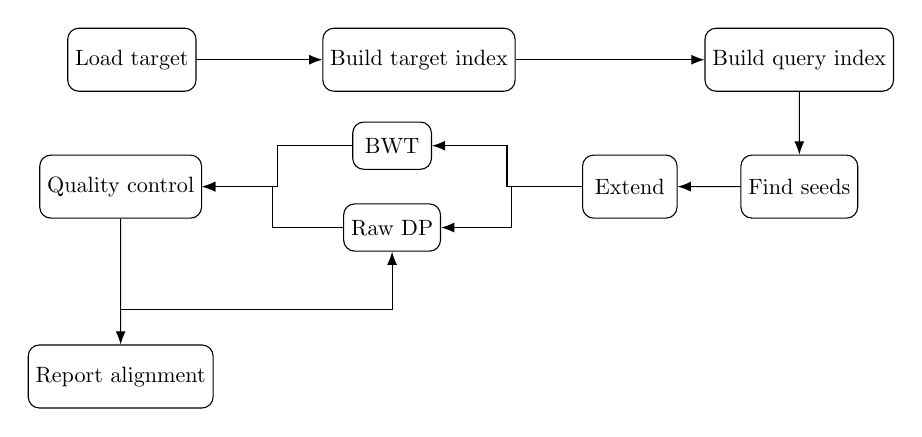
\begin{tikzpicture}[scale=.8, transform shape, node distance=1cm, >=Latex]
    \node(LT)[bigbox]{Load target};
    \node(TI)[bigbox, right=2cm of LT]{Build target index};
    \node(LQ)[bigbox, right=3cm of TI]{Build query index};
    \node(S)[bigbox, below=of LQ]{Find seeds};
    \node(E)[bigbox, left=of S]{Extend};


    \node[place](X)[left=3cm of E]{};
    \node(ABWT)[smallbox, above=2.5mm of X]{BWT};
    \node(ADP)[smallbox, below=2.5mm of X]{Raw DP};

    \node(QC)[bigbox, left=3cm of X]{Quality control};
    \node(R)[bigbox, below=2cm of QC]{Report alignment};

    \draw[->](LT)--(TI);
    \draw[->](TI)--(LQ);
    \draw[->](LQ)--(S);
    \draw[->](S)--(E);
    \draw[->](QC)--(R);

    \draw[fork](E.west)--(ABWT.east);
    \draw[fork](E.west)--(ADP.east);

    \draw[fork](ABWT.west)--(QC.east);
    \draw[fork](ADP.west)--(QC.east);

    %\draw[fork](QC.south)--(ADP.south);

    \path ($(R)!0.45!(ADP)$) -| (QC) coordinate [pos=0.2] (aux);
    \draw (QC) |- (aux);
    \draw[->] (aux) -| (ADP);

  \end{tikzpicture}
  \par}
\end{frame}

\begin{frame}
  \frametitle{Aligner algorithm description}
  \scriptsize
  \begin{enumerate}
    \item Build reference index structures
    \begin{enumerate}
      \scriptsize
      \item Read reference in chunks of size $800000$
      \item For each chunk generate (k=$17$, w=$8$)-minimizer index chunk
      \item Filter out every other $15$-th k-mer (only if it occurs only once within the chunk)
      \item Merge chunk index into full reference index and repeat for other chunks
    \end{enumerate}
    \item Load query and build (k=$17$, w=$8$)-minimizer index
    \item Find common matches and generate cross-product
    \item Perform seed extension (described in detail later) and generate matching positions with scores
    \item Filter $5$ top scores $\geq 0.1$
    \begin{enumerate}
        \scriptsize
        \item For $|scores| = 0$ try building full LIS and use sliding window with highest scoring: $min(|match_q|, |match_t|)^2 - \sum {diff(match_t)}$
        \item For $|scores| = 1$ proceed normally
        \item For $|scores| > 1$ get region with lowest score generated by DP aligner
    \end{enumerate}
    \item Perform final one region matching
  \end{enumerate}

\end{frame}


\begin{frame}
  \frametitle{Aligner algorithm description}
  \scriptsize
  \begin{enumerate}
    \setcounter{enumi}{5}
    \item Perform final one region matching
    \begin{enumerate}
      \scriptsize
      \item For every region virtually resize it by $kmer\_len*0.5+1 = 9$ each side
      \item For every region do quick BWT backtrack aligment on $10\%$ of match (start and end) with max err. rate $10\%=10$
      \item If BWT finds match on end but padding exceeds $4\%$ of match length, execute DP aligner (but only on first parameter configuration i.e $(15, 11)$)
      \begin{enumerate}
        \scriptsize
        \item DP aligner takes prefix/suffix of $40\%$ of query size
        \item For $(kmer_len, step) = ((15, 11), (8, 5))$ it tries to match the pair target/sequence
        \item Run recursive algorithm with threshold of errors $\leq (|query| * 11.11\%)$
      \end{enumerate}
      \item Now if padding returned by BWT or/and DP aligners make region exceed size of $|query|*105\%$ then repeat BWT matching process with new estimate $start = found\_end - |query|$
      \item If we repeated procedure of running BWT/DP twice and came here again, then we assume there is no good match
    \end{enumerate}
    \item Filter out matches if region exceed size of $|query|*105\%$
    \item Print matches coorindates
  \end{enumerate}

\end{frame}

\begin{frame}[fragile]
  \frametitle{Minimizer generation i.e numpy magic}

  \begin{minted}[fontsize=\scriptsize]{python}
  def get_minimizers(seq_arr: NDArray[Shape["*"], UInt8]): 
      sequence_len = len(seq_arr)
      mask = generate_mask(KMER_LEN)  # Bitwise mask

      # Function to compute kmer value based on the previous
      # (on the left side) kmer value and new nucleotide
      uadd = frompyfunc(lambda x, y: ((x << 2) | y) & mask, 2, 1)
      kmers = uadd.accumulate(seq_arr, dtype=object).astype(int)
      kmers[:KMER_LEN-2] = 0
      
      # Do sliding window and get min kmers positions
      kmers_min_pos = add(
          argmin(
            sliding_window_view(kmers, window_shape=WINDOW_LEN
          ), axis=1),
          arange(0, sequence_len - WINDOW_LEN + 1)
      )
      
      # ...
  \end{minted}
\end{frame}

\begin{frame}[fragile]
  \frametitle{Minimizer generation i.e numpy magic}

  \begin{minted}[fontsize=\tiny]{python}
      # ...
      # Now collect all selected mimumum and kmers into single table
      selected_kmers = column_stack((
        kmers[kmers_min_pos],
        kmers_min_pos,
      ))[KMER_LEN:].astype(uint32)

      # Remove duplicates
      selected_kmers = selected_kmers[selected_kmers[:, 0].argsort()]
      selected_kmers = unique(selected_kmers, axis=0)

      # This part performs "group by" using the kmer value
      selected_kmers_unique_idx = unique(
        selected_kmers[:, 0], return_index=True
      )[1][1:]
      selected_kmers_entries_split = split(selected_kmers[:, 1], selected_kmers_unique_idx)

      if len(selected_kmers) == 0:
          return dict()
      return dict(zip(
        chain([selected_kmers[0, 0]], selected_kmers[selected_kmers_unique_idx, 0]),
        selected_kmers_entries_split
      ))
  \end{minted}
\end{frame}

\begin{frame}
  \frametitle{Problem of extending seeds}

  \begin{itemize}
    \item minimap2 approach with dynamic programming similar to normal alignment (plus exponential forward lookups)
    \item We have only one potential match so maybe assume that $match \in LIS(matches)$
    \item Can we formulate sliding window approach to generate the biggest scorring windows included in $LIS(matches)$?
    \item For which case assumption that $match \in LIS(matches)$ won't work?
    \item Can we modify LIS to perhaps include other potential matches?
  \end{itemize}
\end{frame}

\begin{frame}
  \frametitle{Seed extension}
  
  \begin{algorithm}[H]
      \captionsetup{font=scriptsize}
      \caption{Standard LIS construction O(n log n)}\label{alg:cap}
      \scriptsize
      \begin{algorithmic}
          \Require $n \geq 0$
          %\Ensure $y = x^n$
          \State $lis\_len \gets 0$ \Comment{Length of LIS}
          \State $parent \gets \{\infty, \infty, \infty, ..., \infty\}_{n+1}$ \Comment{Mapping to reconstruct LIS}
          \State $sub \gets \{\infty, \infty, \infty, ..., \infty\}_{n+1}$ \Comment{Array with indices for matches that form LIS}
          \State $i \gets 0$
          \While{$i < n$} \Comment{Iterate over all elements $i = 0, 1, 2..., n-1$}
              \State $start \gets 1$
              \State $end \gets lis\_len$
              \While{$start \leq end$} \Comment{Binary search over existing longest sequence}
                  \State $middle \gets \floor*{\frac{start + end}{2}}$
                  \If{$matches_{q}[sub[middle]] < matches_{q}[i]$}
                      \State{$start \gets middle + 1$}
                  \Else
                      \State{$start \gets middle - 1$}
                  \EndIf
              \EndWhile
              \State{$parent[i] \gets sub[start-1]$} \Comment{We pin current value to the found parent}
              \State{$sub[start] \gets i$}
              \If{$start > lis\_len$}
                  \State{$lis\_len = start$}
              \EndIf
              \State{$i \gets i+1$}
          \EndWhile
      \end{algorithmic}
  \end{algorithm}
\end{frame}

\begin{frame}
  \frametitle{Seed extension}
  \begin{algorithm}[H]
    \caption{Reconstruct LIS by following parent array O(n)}\label{alg:cap}
    \begin{algorithmic}
        \State{$current\_node \gets sub[lis\_len]$}
        \State{$result \gets \{0, 0, 0,..., 0\}_{lis\_len}$}
        \State{$result[lis\_len-1] \gets current\_node$} \Comment{Will contain all indices from matches describing the output subsequence}
        \State{$j \gets lis\_len-1 $}
        \While{$1 \leq j$}
            \State{$current\_node \gets parent[current\_node]$}
            \State{$result[j-1] \gets current\_node$}
            \State{$j \gets j-1$}
        \EndWhile
    \end{algorithmic}
  \end{algorithm}
\end{frame}

\begin{frame}[fragile]
  \frametitle{Seed extension (unwanted case)}

  \begin{center}
    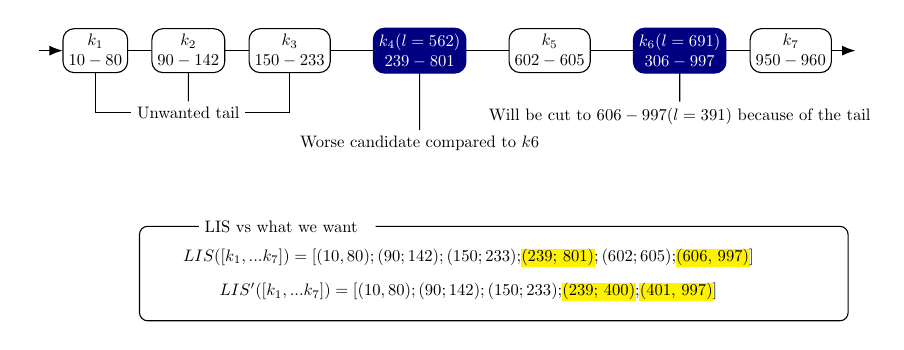
\begin{tikzpicture}[scale=.6, transform shape, node distance=1cm, >=Latex, remember picture]

      \node(kstart)[]{};
      \node(k1)[tinybox, right=0.5cm of kstart, align=center]{$k_1$\\$10-80$};
      \node(k2)[tinybox, right=0.5cm of k1, align=center]{$k_2$\\$90-142$};
      \node(k3)[tinybox, right=0.5cm of k2, align=center]{$k_3$\\$150-233$};
      \node(k4)[tinybox, colprimary, right=0.9cm of k3, align=center]{$k_4 (l=562)$\\$239-801$};
      \node(k5)[tinybox, right=0.9cm of k4, align=center]{$k_5$\\$602-605$};
      \node(k6)[tinybox, colprimary, right=0.9cm of k5, align=center]{$k_6 (l=691)$\\$306-997$};
      \node(k7)[tinybox, right=0.5cm of k6, align=center]{$k_7$\\$950-960$};
      \node(kend)[right=0.5cm of k7]{};
  
      \draw[->](kstart)--(k1);
      \draw[-](k1)--(k2);
      \draw[-](k2)--(k3);
      \draw[-](k3)--(k4);
      \draw[-](k4)--(k5);
      \draw[-](k5)--(k6);
      \draw[-](k6)--(k7);
      \draw[->](k7)--(kend);
  
      \node(desctail)[below=0.6cm of k2]{Unwanted tail};
      \draw (k1) |- (desctail.west);
      \draw (k2) -- (desctail.north);
      \draw (k3) |- (desctail.east);
  
      \node(desck4)[below=1.2cm of k4]{Worse candidate compared to $k6$};
      \draw (k4) -- (desck4.north);
  
      \node(desck6)[below=0.6cm of k6]{Will be cut to $606-997 (l=391)$ because of the tail};
      \draw (k6) -- (desck6.north);
  
      \node (listitle)[below right=3cm and 1.5cm of k1]{LIS vs what we want};
      \draw[rounded corners=3pt]
      (listitle) -| ++(-3cm, -2cm) coordinate(listitle) -| ++(15cm, 2cm) coordinate(listitle) -- ++(-10cm, 0cm) coordinate(listitle);
  
      \node(listext1)[below right=0.35cm and -4.2cm of listitle]{$LIS([k_1,...k_7]) = [ (10, 80); (90; 142); (150; 233); $\hl{(239; 801)}$; (602; 605); $\hl{(606, 997)}$ ]$};
  
      \node(listext2)[below=0.1cm of listext1]{$LIS'([k_1,...k_7]) = [ (10, 80); (90; 142); (150; 233); $\hl{(239; 400)}$; $\hl{(401, 997)}$ ]$};
      
    \end{tikzpicture}
  \end{center}

\end{frame}

\begin{frame}
  \frametitle{Seed extension (heuristic)}
  
  \begin{algorithm}[H]
      \captionsetup{font=scriptsize}
      \caption{Segmented-LIS heuristic O(n log n)}\label{alg:cap}
      \tiny
      \begin{algorithmic}
          \Require $n \geq 0$
          %\Ensure $y = x^n$
          \State $lis\_len \gets 0$ \Comment{Length of LIS}
          \State $parent \gets \{\infty, \infty, \infty, ..., \infty\}_{n+1}$ \Comment{Mapping to reconstruct LIS}
          \State $sub \gets \{\infty, \infty, \infty, ..., \infty\}_{n+1}$ \Comment{Array with indices for matches that form LIS}
          \State $i \gets 0$
          \While{$i < n$} \Comment{Iterate over all elements $i = 0, 1, 2..., n-1$}
              \State $start \gets 1$
              \State $end \gets lis\_len$
              \While{$start \leq end$} \Comment{Binary search-like}
                  \State $middle \gets \floor*{\frac{start + end}{2}}$
                  \If{$matches_{T}[sub[middle]] > matches_{T}[i] - max\_diff$} \Comment{Encountered old entry}
                      \State{$end \gets start - 1$} \Comment{Breaks loop}
                  \ElsIf{$matches_{Q}[sub[middle]] < matches_{Q}[i]$}
                      \State{$start \gets middle + 1$}
                  \Else
                      \State{$start \gets middle - 1$}
                  \EndIf
              \EndWhile
              \State{$parent[i] \gets sub[start-1]$} \Comment{We pin current value to the found parent}
              \State{$sub[start] \gets i$}
              \If{$start > lis\_len$}
                  \State{$lis\_len = start$}
              \EndIf
              \State{$i \gets i+1$}
          \EndWhile
      \end{algorithmic}
  \end{algorithm}
\end{frame}

\begin{frame}
  \frametitle{Why does it seems to be working?}

  \begin{itemize}
    \item The case when normal LIS does not work is first worse match with long tail of occurences beforehand
    \item Finishing binary-search early on the left side makes us reuse previous sequences, the more right selections we made
    \item So for each turn right our probability increases
    \item Hence for 3 good matches we will have a high chance of at least having its part in the final array
    \item Of course with increasing numer of candidates (especially with lower starting positions) it will work worse and worse
  \end{itemize}
\end{frame}

\begin{frame}
  \frametitle{What after we generated LIS heuristic?}

  \begin{itemize}
    \item We can do the sliding window technique as query indices will be monotonic (locally) after we encounter target gap
    \item Hence we can formulate simple algorithm for each starting position $i$ in our heuristical-LIS array
    \begin{enumerate}
        \item For each $i$ find last available target position $j$ (using binary search)
        \item For window we define $spaces(s) = \sum_{\substack{k \in \{1,2,...,f\},\\match[k] \in window [i, j]}} {(\frac{min(match[k]_s-match[k-1]_s, kmer\_len)}{kmer\_len})}$
        \item Calculate window score using: $score \gets \frac{min(|match_q|, |match_t|) - max(spaces_t, spaces_q)}{|query|}$
        \item If the score is local maximum i.e $score_{i-1} < score_{i} \land (score_{i} > score{i+1} \lor i+1 == |LIS|)$ then add it to the max scores bucket $max\_scores[\frac{i}{|query|*10\%}] \gets max\_scores[\frac{i}{|query|*10\%}] \cup \{score_{i}\}$
    \end{enumerate}
    \item Filter $5$ top scores $\geq 0.1$ (see previous slides)
  \end{itemize}
\end{frame}



\begin{frame}[fragile]
  \frametitle{Execution times}
  \begin{figure}[ht]
    \centering
    \begin{CacheMeCode}{python, custom include command={\input{\robExtAddCachePathAndName{\robExtFinalHash.pgf}}}, set placeholder eval={__LINEWIDTH__}{\lenToCmNoUnit[in]{\linewidth}}}
      import matplotlib.pyplot as plt
      import matplotlib
      import numpy as np
      import json
      matplotlib.use("pgf")
      matplotlib.rcParams.update({
        "font.family": "serif",
        "font.serif": [],
        "text.usetex": True,
      })
      with open('../experiments_data.json') as f:
          stats = json.load(f)
      fig, ax = plt.subplots()
      fig.set_size_inches(__LINEWIDTH__, 0.6*__LINEWIDTH__, forward=True)
      #cases = sorted(list({case_name for program_label, program_stats in stats.items() for case_name in program_stats if "read_bwt_pad_begin" in program_stats[case_name]}))
      cases = ["20Ma", "20Mb", "small_reads1"]
      program_label_mapping = {
        "solution": "solution",
      }
      width = 0.3
      multiplier = 0
      x = np.arange(len(cases))
      color_per_solution = {
        "solution": "#ED0020",
      }

      for program_label, program_stats in stats.items():
        if program_label in program_label_mapping:
          offset = width * multiplier

          vals_index_target = [(program_stats[case]["ref_chunk_building"]["t_total"] if "ref_chunk_building" in program_stats[case] else 0)/1000 for case in cases]
          vals_index_query = [(program_stats[case]["read_index_building"]["t_total"] if "read_index_building" in program_stats[case] else 0)/1000 for case in cases]
          vals_read_lis = [(program_stats[case]["read_lis"]["t_total"] if "read_lis" in program_stats[case] else 0)/1000 for case in cases]
          vals_read_lis_cutoff = [(program_stats[case]["read_lis_cutoff"]["t_total"] if "read_lis_cutoff" in program_stats[case] else 0)/1000 for case in cases]
          vals_read_bwt = [(program_stats[case]["read_bwt"]["t_total"] if "read_bwt" in program_stats[case] else 0)/1000 for case in cases]
          vals_read_dp = [(program_stats[case]["read_dp"]["t_total"] if "read_dp" in program_stats[case] else 0)/1000 for case in cases]

          bottom = [0 for i in vals_index_query]
          for (series, color, name) in [
            (vals_index_target, "#ED0020", "Index target"),
            (vals_index_query, "#107AB0", "Index query"),
            (vals_read_lis, "#FFDE21", "Read LIS"),
            (vals_read_lis_cutoff, "#006A4E", "Find best LIS region"),
            (vals_read_bwt, "#33006F", "BWT Alignment"),
            (vals_read_dp, "#F96D00", "DP Alignment"),
          ]:
            ax.bar(x + offset, series, width, bottom=bottom, color=color, label=f"{program_label_mapping[program_label]}: {name}")
            bottom = [bottom[i]+series[i] for i in range(len(bottom))]
          # ax.bar(x + offset, vals_index_target, width, bottom=vals_index_query,  color="#107AB0", label=f"{program_label_mapping[program_label]}: Index target")
          # ax.bar(x + offset, vals_read_lis, width, bottom=vals_index_target, color="#FFDE21", label=f"{program_label_mapping[program_label]}: Read LIS")
          # ax.bar(x + offset, vals_read_lis_cutoff, width, bottom=vals_read_lis, color="#006A4E", label=f"{program_label_mapping[program_label]}: Find best LIS region")
          # ax.bar(x + offset, vals_read_align, width, bottom=vals_read_lis_cutoff, color="#33006F", label=f"{program_label_mapping[program_label]}: Alignments")
          multiplier += 1
          offset = width * multiplier
          
          #end=[program_stats[case]["read_bwt_pad_end"]["t_total"] for case in cases],
          #), width, label="st-"+program_label_mapping[program_label])
          #ax.bar_label(rects, padding=3)
          #multiplier += 1

      ax.set_xticks(x + width/2)
      ax.set_xticklabels([case.replace('_', '-') for case in cases])
      ax.set_ylabel('Total runtime [s]', fontsize=8)
      #ax.set_yscale("log")
      ax.set_title("Total runtime by category", fontsize=8)
      ax.legend(loc='upper center', bbox_to_anchor=(0.5, -0.2),
          ncol=2, fancybox=False, shadow=False, prop={'size': 6}, frameon=False)

      print(get_filename_from_extension(".pgf"))
      plt.savefig(get_filename_from_extension(".pgf"), bbox_inches="tight")
    \end{CacheMeCode}
  \end{figure}
\end{frame}

\begin{frame}[fragile]
  \frametitle{Aligner routine effectiveness}
  \begin{figure}[ht]
    \centering
    \begin{CacheMeCode}{python, custom include command={\input{\robExtAddCachePathAndName{\robExtFinalHash.pgf}}}, set placeholder eval={__LINEWIDTH__}{\lenToCmNoUnit[in]{\linewidth}}}
      import matplotlib.pyplot as plt
      import matplotlib
      import numpy as np
      import json
      matplotlib.use("pgf")
      matplotlib.rcParams.update({
        "font.family": "serif",
        "font.serif": [],
        "text.usetex": True,
      })
      with open('../experiments_data.json') as f:
          stats = json.load(f)
      b = 2
      fig, ax = plt.subplots()
      fig.set_size_inches(__LINEWIDTH__, 0.6*__LINEWIDTH__, forward=True)
      #cases = sorted(list({case_name for program_label, program_stats in stats.items() for case_name in program_stats if "read_bwt_pad_begin" in program_stats[case_name]}))
      cases = ["20Ma", "20Mb"]
      program_label_mapping = {
        "solution": "10% ER=10%",
        "bwt-fragment-02p01": "20% ER=10%",
        "bwt-fragment-03p006": "30% ER=6%",
        "bwt-fragment-03p008": "30% ER=8%",
      }
      width = 0.25
      multiplier = 0
      x = np.arange(len(cases))
      color_per_solution = {
        "solution": "#ED0020",
        "bwt-fragment-02p01": "#107AB0",
        "bwt-fragment-03p006": "#FFDE21",
        "bwt-fragment-03p008": "#006A4E",
      }

      for program_label, program_stats in stats.items():
        if program_label in program_label_mapping:
          offset = width * multiplier
          vals_start = [(program_stats[case]["read_bwt_pad_begin"]["t_total"] if "read_bwt_pad_begin" in program_stats[case] else 0) for case in cases]
          vals_end = [(program_stats[case]["read_bwt_pad_end"]["t_total"] if "read_bwt_pad_end" in program_stats[case] else 0) for case in cases]
          rects = ax.bar(x + offset, vals_start, width, hatch="0", label=f"{program_label_mapping[program_label]} (R)", color=color_per_solution[program_label], edgecolor=color_per_solution[program_label])
          ax.bar(x + offset, vals_end, width, bottom=vals_start, hatch="//", color="white", edgecolor=color_per_solution[program_label], label=f"{program_label_mapping[program_label]} (L)")
          #end=[program_stats[case]["read_bwt_pad_end"]["t_total"] for case in cases],
          #), width, label="st-"+program_label_mapping[program_label])
          ax.bar_label(rects, padding=3)
          multiplier += 1

      ax.set_xticks(x + width/2)
      ax.set_xticklabels([case.replace('_', '-') for case in cases])
      ax.set_ylabel('Total BWT matches per file', fontsize=8)
      ax.set_title("Number of paddings adjusted via BWT", fontsize=8)
      ax.legend(loc='upper center', bbox_to_anchor=(0.4, -0.2),
          ncol=4, fancybox=False, shadow=False, prop={'size': 6}, frameon=False)

      print(get_filename_from_extension(".pgf"))
      plt.savefig(get_filename_from_extension(".pgf"), bbox_inches="tight")
    \end{CacheMeCode}
  \end{figure}
\end{frame}

\begin{frame}[fragile]
  \frametitle{BWT routine implementation}
  \begin{figure}[ht]
    \centering
    \begin{CacheMeCode}{python, custom include command={\input{\robExtAddCachePathAndName{\robExtFinalHash.pgf}}}, set placeholder eval={__LINEWIDTH__}{\lenToCmNoUnit[in]{\linewidth}}}
      import matplotlib.pyplot as plt
      import matplotlib
      import numpy as np
      import json
      matplotlib.use("pgf")
      matplotlib.rcParams.update({
        "font.family": "serif",
        "font.serif": [],
        "text.usetex": True,
      })
      with open('../experiments_data.json') as f:
          stats = json.load(f)
      fig, ax = plt.subplots()
      fig.set_size_inches(__LINEWIDTH__, 0.7*__LINEWIDTH__, forward=True)
      cases = sorted(list({case_name for program_label, program_stats in stats.items() for case_name in program_stats}))
      program_label_mapping = {
        "solution": "bwt-naive",
        "bwt-dp-numpy": "bwt-skew-numpy",
        "bwt-dp-lists": "bwt-skew-lists",
      }
      width = 0.25
      multiplier = 0
      x = np.arange(len(cases))
      for program_label, program_stats in stats.items():
        if program_label in program_label_mapping:
          offset = width * multiplier
          rects = ax.bar(x + offset, [program_stats[case]["read_bwt"]["t_avg"] for case in cases], width, label=program_label_mapping[program_label])
          ax.bar_label(rects, padding=3)
          multiplier += 1

      ax.set_xticks(x + width/2)
      ax.set_xticklabels([case.replace('_', '-') for case in cases])
      ax.set_ylabel('Execution time/query [ms]')
      ax.set_title("BWT subroutine execution time")
      ax.legend(title='Program')

      print(get_filename_from_extension(".pgf"))
      plt.savefig(get_filename_from_extension(".pgf"), bbox_inches="tight")
    \end{CacheMeCode}
  \end{figure}
\end{frame}



\begin{frame}[fragile]
  \frametitle{Raw DP routine implementation}
  \begin{figure}[ht]
    \centering
    \begin{CacheMeCode}{python, custom include command={\input{\robExtAddCachePathAndName{\robExtFinalHash.pgf}}}, set placeholder eval={__LINEWIDTH__}{\lenToCmNoUnit[in]{\linewidth}}}
      import matplotlib.pyplot as plt
      import matplotlib
      import numpy as np
      import json
      matplotlib.use("pgf")
      matplotlib.rcParams.update({
        "font.family": "serif",
        "font.serif": [],
        "text.usetex": True,
      })
      with open('../experiments_data.json') as f:
          stats = json.load(f)
      fig, ax = plt.subplots()
      fig.set_size_inches(__LINEWIDTH__, 0.7*__LINEWIDTH__, forward=True)
      cases = sorted(list({case_name for program_label, program_stats in stats.items() for case_name in program_stats if "read_dp" in program_stats[case_name]}))
      program_label_mapping = {
        "solution": "dp-lists",
        "bwt-dp-numpy": "dp-numpy",
      }
      width = 0.25
      multiplier = 0
      x = np.arange(len(cases))
      for program_label, program_stats in stats.items():
        if program_label in program_label_mapping:
          offset = width * multiplier
          rects = ax.bar(x + offset, [program_stats[case]["read_dp"]["t_total"] for case in cases], width, label=program_label_mapping[program_label])
          ax.bar_label(rects, padding=3)
          multiplier += 1

      ax.set_xticks(x + width/2)
      ax.set_xticklabels([case.replace('_', '-') for case in cases])
      ax.set_ylabel('Execution time (total) [ms]')
      ax.set_title("DP subroutine execution time")
      ax.legend(title='Program')

      print(get_filename_from_extension(".pgf"))
      plt.savefig(get_filename_from_extension(".pgf"), bbox_inches="tight")
    \end{CacheMeCode}
  \end{figure}
\end{frame}


\begin{frame}
  \frametitle{Match quality evaluation}

  Assuming we have match $(r_1, r_2)$ and expect $(e_1, e_2)$
  We define the following:

  \begin{itemize}
    \item $d_1 \coloneqq |e_1 - r_1|$
    \item $d_2 \coloneqq |e_2 - r_2|$
    \item $d_s \coloneqq d_1 + d_2$
    \item $d_m \coloneqq max(d_1, d_2)$
  \end{itemize}

  \begin{itemize}
    \item $score((r_1, r_2)) = AA$ iff $d_s < 10$
    \item $score((r_1, r_2)) = AB$ iff $d_s < 20$
    \item $score((r_1, r_2)) = C$ iff $d_m < 20$
    \item $score((r_1, r_2)) = D$ iff $d_m \geq 20$
  \end{itemize}

  
  \begin{table}[]
    \begin{tabular}{|l|l|l|l|l|l|l|}
    \hline
    case name                        & ok                          & unmapped                 & AA                         & AB                        & C                        & D (bad)                  \\ \hline
    \rowcolor[HTML]{333333} 
    {\color[HTML]{FFFFFF} reads20Mb} & {\color[HTML]{FFFFFF} 1000} & {\color[HTML]{FFFFFF} 0} & {\color[HTML]{FFFFFF} 936} & {\color[HTML]{FFFFFF} 64} & {\color[HTML]{FFFFFF} 0} & {\color[HTML]{FFFFFF} 0} \\ \hline
    \rowcolor[HTML]{FFFFFF} 
    {\color[HTML]{333333} reads20Ma} & {\color[HTML]{333333} 1000} & {\color[HTML]{333333} 0} & {\color[HTML]{333333} 975} & {\color[HTML]{333333} 25} & {\color[HTML]{333333} 0} & {\color[HTML]{333333} 0} \\ \hline
    \rowcolor[HTML]{333333} 
    {\color[HTML]{DAE8FC} reads2}    & {\color[HTML]{DAE8FC} 100}  & {\color[HTML]{DAE8FC} 0} & {\color[HTML]{DAE8FC} 90}  & {\color[HTML]{DAE8FC} 10} & {\color[HTML]{DAE8FC} 0} & {\color[HTML]{DAE8FC} 0} \\ \hline
    \end{tabular}
  
  \end{table}

\end{frame}

\begin{frame}{}
  \centering \Large
  \emph{Thank you}
\end{frame}

% \begin{frame}[fragile]
%   \frametitle{Sample frame title}

%   \begin{tikzpicture}[
%     scale=5,
%     axis/.style={very thick, ->, >=stealth'},
%     important line/.style={thick},
%     dashed line/.style={dashed, thin},
%     pile/.style={thick, ->, >=stealth', shorten <=2pt, shorten
%     >=2pt},
%     every node/.style={color=black}
%     ]
%     % axis
%     \draw[axis] (-0.1,0)  -- (1.1,0) node(xline)[right]
%         {$Q = (q_1,q_2,...,q_n)$};
%     \draw[axis] (0,-0.1) -- (0,1.1) node(yline)[above] {$T = (t_1,t_2,...,t_m)$};
%     % Lines
%     % \newcommand\kmershift{.10}
%     % \foreach \x in {0,...,4}
%     %   {\draw[important line] (\x*\kmershift+\randeq{.15},\x*\kmershift+\randeq{.15}) coordinate (A) -- (\x*\kmershift+\randeq{.20},\x*\kmershift+\randeq{.20})
%     %       coordinate (B) node[right, text width=1cm] {$k_\x$};}

%     \newcommand\kmershift{.08}
%     \foreach \x in {0,...,6}
%       {
%         \pgfmathsetmacro{\offset}{0.03}
%         \pgfmathsetmacro{\loffset}{0.5}
%         \pgfmathsetmacro{\da}{.15+random(-100,100)/100*\offset};
%         \pgfmathsetmacro{\dy}{.15+random(-100,100)/100*\offset};
%         \pgfmathsetmacro{\xa}{\x*\kmershift+\da};
%         \pgfmathsetmacro{\ya}{\x*\kmershift+\dy};
%         \pgfmathsetmacro{\xb}{\xa+0.05};
%         \pgfmathsetmacro{\yb}{\ya+0.05};
%         \draw[important line] (\xa,\ya) coordinate (A) -- (\xb,\yb)
%           coordinate (B) node[right=\offset of A, font=\small] {$k_\x$};}
%     \foreach \x in {7,...,9}
%       {
%         \pgfmathsetmacro{\offset}{0.03}
%         \pgfmathsetmacro{\loffset}{0.5}
%         \pgfmathsetmacro{\da}{.52+random(-100,100)/100*\offset};
%         \pgfmathsetmacro{\dy}{.70+random(-100,100)/100*\offset};
%         \pgfmathsetmacro{\xa}{(\x-7)*\kmershift+\da};
%         \pgfmathsetmacro{\ya}{(\x-7)*\kmershift+\dy};
%         \pgfmathsetmacro{\xb}{\xa+0.05};
%         \pgfmathsetmacro{\yb}{\ya+0.05};
%         \draw[important line] (\xa,\ya) coordinate (A) -- (\xb,\yb)
%           coordinate (B) node[right=\offset of A, font=\small] {$k_\x$};}
%     \foreach \x in {10,...,15}
%     {
%       \pgfmathsetmacro{\offset}{0.03}
%       \pgfmathsetmacro{\xa}{(\x-10)*0.1+0.3+random(0,100)/100*0.03};
%       \pgfmathsetmacro{\ya}{\xa*random(20,60)/100};
%       \pgfmathsetmacro{\xb}{\xa+0.05};
%       \pgfmathsetmacro{\yb}{\ya+0.05};
%       \draw[important line] (\xa,\ya) coordinate (A) -- (\xb,\yb)
%         coordinate (B) node[right=\offset of A, font=\small] {$k_{\x}$};}

%     % \draw[important line] (.15,.85) coordinate (C) -- (.85,.15)
%     %     coordinate (D) node[right, text width=5em] {$\mathit{NX}=x$};
%     % Intersection of lines
%     % \fill[red] (intersection cs:
%     %    first line={(A) -- (B)},
%     %    second line={(C) -- (D)}) coordinate (E) circle (.4pt)
%     %    node[above,] {$A$};
%     % % The E point is placed more or less randomly
%     % \fill[red]  (E) +(-.075cm,-.2cm) coordinate (out) circle (.4pt)
%     %     node[below left] {$B$};
%     % % Line connecting out and ext balances
%     % \draw [pile] (out) -- (intersection of A--B and out--[shift={(0:1pt)}]out)
%     %     coordinate (extbal);
%     % \fill[red] (extbal) circle (.4pt) node[above] {$C$};
%     % % line connecting  out and int balances
%     % \draw [pile] (out) -- (intersection of C--D and out--[shift={(0:1pt)}]out)
%     %     coordinate (intbal);
%     % \fill[red] (intbal) circle (.4pt) node[above] {$D$};
%     % % line between out og all balanced out :)
%     % \draw[pile] (out) -- (E);
%   \end{tikzpicture}
% \end{frame}

\end{document}


% % Local Variables:
% % TeX-command-extra-options: "--shell-escape -halt-on-error"
% % End: